% 5:30 - 6:45  = 75 minutes
% skipped 1 for of the questions, 33% penalty
% 100 minutes

\begin{solutionbox}[Q2-1]
    \begin{center}
        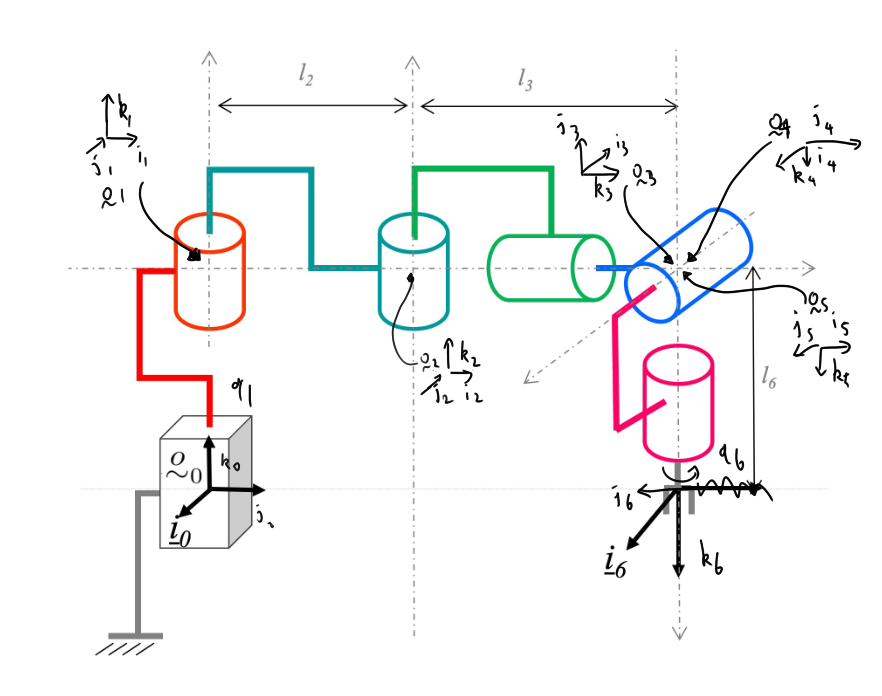
\includegraphics[width=120mm]{imgs/y2023-v1-q2.png}
    \end{center}

    \begin{center}
        \begin{tabular}{lllll}
               & $\theta$           & $d$   & $a$   & $\alpha$ \\
            j0 & $\pi/2$            & $d_1$ & 0     & 0        \\
            j1 & $\theta_2$         & 0     & $l_2$ & 0        \\
            j2 & $\pi/2+\theta_3$   & 0     & $l_3$ & $\pi/2$  \\
            j3 & $ -\pi/2+\theta_4$ & 0     & 0     & $\pi/2$  \\
            j4 & $\pi/2+\theta_5$   & 0     & 0     & $\pi/2$  \\
            j5 & $\pi/2$            & $l_6$ & 0     & 0        \\
        \end{tabular}
    \end{center}

    \begin{align*}
        {\,^0T_1} & =
        \begin{bmatrix}
            [e^{\frac{\pi}{2} k \times}] & [d_1 k] \\
            [0]                          & 1
        \end{bmatrix}
    \end{align*}

    \begin{align*}
        {\,^1T_2} & =
        \begin{bmatrix}
            [e^{\theta_2 k \times}] & [0] \\
            [0]                     & 1
        \end{bmatrix}
        \begin{bmatrix}
            [I_3] & [l_2 i] \\
            [0]   & 1
        \end{bmatrix} \\
                  & =
        \begin{bmatrix}
            [e^{\theta_2 k \times}] & [e^{\theta_2 k \times} \cdot l_2 i    ] \\
            [0]                     & 1
        \end{bmatrix}
    \end{align*}

    \begin{align*}
        {\,^2T_3} & =
        \begin{bmatrix}
            [e^{(\pi/2+\theta_3) k \times}] & [0] \\
            [0]                             & 1
        \end{bmatrix}
        \begin{bmatrix}
            [e^{(\pi/2) i \times}] & [l_3 i] \\
            [0]                    & 1
        \end{bmatrix} \\
                  & =
        \begin{bmatrix}
            [e^{(\pi/2+\theta_3) k \times}e^{(\pi/2) i \times}] & [e^{(\pi/2+\theta_3) k \times} l_3 i] \\
            [0]                                                 & 1
        \end{bmatrix}
    \end{align*}

    \begin{align*}
        {\,^3T_4} & =
        \begin{bmatrix}
            [e^{(-\pi/2. +\theta_4) k \times}] & [0] \\
            [0]                                & 1   \\
        \end{bmatrix}
        \begin{bmatrix}
            [e^{(\pi/2) i \times}] & [0] \\
            [0]                    & 1
        \end{bmatrix} \\
                  & =
        \begin{bmatrix}
            [e^{(-\pi/2. +\theta_4) k \times}e^{(\pi/2) i \times}] & [0] \\
            [0]                                                    & 1   \\
        \end{bmatrix}
    \end{align*}

    \begin{align*}
        {\,^4T_5} & =
        \begin{bmatrix}
            [e^{(\pi/2. +\theta_5) k \times}] & [0] \\
            [0]                               & 1   \\
        \end{bmatrix}
        \begin{bmatrix}
            [e^{(\pi/2) i \times}] & [0] \\
            [0]                    & 1
        \end{bmatrix} \\
                  & =
        \begin{bmatrix}
            [e^{(\pi/2. +\theta_5) k \times}e^{(\pi/2) i \times}] & [0] \\
            [0]                                                   & 1   \\
        \end{bmatrix}
    \end{align*}

    \begin{align*}
        {\,^5T_6} & =
        \begin{bmatrix}
            [e^{\pi/2 k \times}] & [l_6 k] \\
            [0]                  & 1
        \end{bmatrix}
    \end{align*}
\end{solutionbox}

\begin{solutionbox}[Q2-2]
    \footnotesize
    \begin{align*}
        J & =
        \begin{bmatrix}
            k_0                              &
            k_1 \times (\ppori{6}-\ppori{1}) &
            k_2 \times (\ppori{6}-\ppori{2}) &
            k_3 \times (\ppori{6}-\ppori{3}) &
            k_4 \times (\ppori{6}-\ppori{4}) &
            k_5 \times (\ppori{6}-\ppori{5})   \\
            0                                &
            k_1                              &
            k_2                              &
            k_3                              &
            k_4                              &
            k_5
        \end{bmatrix}
    \end{align*}


    since this is a spherical wrist, the wrist and the arm can be analyzed separately.

    \begin{align*}
        \begin{bmatrix}
            [I_3] & (\ppori{6}-\ppori{3})\times \\
            [0]   & [I_3]
        \end{bmatrix}
        J & =
        \begin{bmatrix}
            k_0                              &
            k_1 \times (\ppori{3}-\ppori{1}) &
            k_2 \times (\ppori{3}-\ppori{2}) &
            0                                &
            0                                &
            0                                  \\
            0                                &
            k_1                              &
            k_2                              &
            k_3                              &
            k_4                              &
            k_5
        \end{bmatrix}
    \end{align*}


    When $\theta_3 = 0$ or $\theta_3 = \pi$, joint 2 and joint 3 have the same effect, so it is a singularity.
    (I forgot this in previous practices.)

    When $\theta_5 = 0$ or $\theta_5=\pi$, joint 4 k axis and joint 6 k axis are aligned, so there effect are the same and is a singularity.

    (the following are probably not right since i'm not sure what suitable means here)

    yes, if the tasks arein one plane, then the first joint does't need to move and saves power. and if all of tasks are in a cylinedarical surface, it would line up with the first two degrees of freedom of the robot.


    The reachable workspace is a cylinder with height equal tot he rang eof the prismatic joint and radius l2, l3, l6, plus two capsules on top and bottom with height l6 flat region bounded outside by l3, bounded inside by radius equal to difference of l2 and l3.

    the dexerous workspace is a cylinder with height therange of the prismatic joint, and radius equal to l2+l3 - l6. th einside is more complicated. for a unreachable radius of |l2-l3|. |l2-l3|+l6 is not dexerous. top and bottom is too messy.

\end{solutionbox}

\begin{solutionbox}[Q2-3]

    walk back wads from o6 by k6 to get to wrist center.

    the height of the wrist center is where d1 is.

    the distance of the wrist center, as well as l2 and l3, can be passed into kahan 4 to solve for theta 3.

    mean of theta 2 can be found with kahan 2 rotating from i2 to o3-o1 using k0.

    using pi minus kahan 4 using a being the magneitude of o3-o1 as a, l2 as b, and l3 as c solves for theta 2 delta.

    both theta 2 delta and theta 3 are plus minus version but theta2 delta and theta 3 should have opposite sign. so the solution space branched into 2.

    project k6 onto i3 and j3 and normalize. the use kahan 2 from j3 to projected k6 around k3 gives one solution for theta 4, adding pi gives another solution for theta 4. so now the solution space has branched into 4.

    given variable up to theta 4, using kahan 2 from i5 to k5 using k4 gives the angle for theta 5. this is unique up to mod 2pi.

    then rotating from j5 to i6 across k5 gives theta 6. also unique.


\end{solutionbox}

\begin{solutionbox}[Q2-4]
    See 2025-v1-q2 last question
\end{solutionbox}